\documentclass[10pt,a4paper]{article}
\newcommand{\ReportShortTitle}{FULL PROJECT DOSSIER}
\usepackage[margin=0.78in]{geometry}
\usepackage{booktabs}
\usepackage{longtable}
\usepackage{array}
\usepackage[table]{xcolor}
\usepackage{enumitem}
\usepackage{tikz}
\usetikzlibrary{positioning,arrows.meta,shapes.geometric,fit,backgrounds,calc}
\usepackage{amsmath}
\usepackage{float}
\usepackage{caption}
\usepackage{fancyhdr}
\usepackage{lastpage}
\usepackage{underscore}
\usepackage[hidelinks]{hyperref}

\definecolor{navy}{HTML}{102A43}
\definecolor{blue}{HTML}{1D70A2}
\definecolor{cyan}{HTML}{2E86AB}
\definecolor{green}{HTML}{2A9D8F}
\definecolor{amber}{HTML}{F4A261}
\definecolor{red}{HTML}{D95D39}
\definecolor{violet}{HTML}{7B61A8}
\definecolor{ink}{HTML}{243B53}
\definecolor{muted}{HTML}{627D98}
\definecolor{paleBlue}{HTML}{EAF4FA}
\definecolor{paleGreen}{HTML}{EAF7F4}
\definecolor{paleAmber}{HTML}{FFF4E6}
\definecolor{grid}{HTML}{CAD8E3}

\newcommand{\stImpl}{\textcolor{green}{\textbf{IMPLEMENTED}}}
\newcommand{\stPartial}{\textcolor{amber!80!black}{\textbf{PARTIAL}}}
\newcommand{\stPlan}{\textcolor{blue}{\textbf{PLANNED}}}
\newcommand{\stGap}{\textcolor{red}{\textbf{GAP}}}
\newcommand{\stBlocked}{\textcolor{red}{\textbf{BLOCKED}}}
\newcommand{\stGate}{\textcolor{violet}{\textbf{GATED}}}
\newcommand{\stVerified}{\textcolor{green}{\textbf{VERIFIED}}}
\newcommand{\code}[1]{\texttt{\small #1}}
\newcommand{\gate}[1]{\textcolor{blue}{\textbf{#1}}}

\newcolumntype{L}[1]{>{\raggedright\arraybackslash}p{#1}}
\newcolumntype{C}[1]{>{\centering\arraybackslash}p{#1}}

\sloppy
\setlength{\emergencystretch}{3em}
\setlength{\parindent}{0pt}
\setlength{\parskip}{5pt}
\setlist[itemize]{leftmargin=1.35em,itemsep=2pt,topsep=3pt}
\setlist[enumerate]{leftmargin=1.55em,itemsep=2pt,topsep=3pt}
\setcounter{tocdepth}{1}
\renewcommand{\arraystretch}{1.18}

\pagestyle{fancy}
\fancyhf{}
\fancyhead[L]{\small\bfseries\textcolor{navy}{SURYAGRID AI}}
\fancyhead[R]{\small\textcolor{muted}{\ReportShortTitle}}
\fancyfoot[L]{\footnotesize\textcolor{muted}{Project Team Document | 9 July 2026}}
\fancyfoot[R]{\footnotesize\textcolor{muted}{Page \thepage\ of \pageref{LastPage}}}
\renewcommand{\headrulewidth}{0.5pt}
\renewcommand{\footrulewidth}{0.4pt}

\tikzset{
  layer/.style={rectangle, rounded corners=2pt, thick, minimum height=1.05cm,
                text width=13.0cm, align=left, font=\small},
  component/.style={rectangle, rounded corners=2pt, draw=blue, fill=paleBlue,
                   text width=2.35cm, minimum height=1.1cm, align=center, font=\scriptsize},
  agent/.style={rectangle, rounded corners=2pt, draw=green, fill=paleGreen,
                text width=2.35cm, minimum height=1.1cm, align=center, font=\scriptsize},
  aiagent/.style={rectangle, rounded corners=2pt, draw=violet, fill=violet!7,
                  text width=2.35cm, minimum height=1.1cm, align=center, font=\scriptsize},
  store/.style={cylinder, shape border rotate=90, aspect=0.28, draw=amber!80!black,
                fill=paleAmber, minimum width=2.25cm, minimum height=1.15cm,
                align=center, font=\scriptsize},
  decision/.style={diamond, aspect=2, draw=amber!80!black, fill=paleAmber,
                   align=center, font=\scriptsize, inner sep=1pt},
  flow/.style={-{Stealth[length=2.2mm]}, thick, draw=navy},
  dataflow/.style={-{Stealth[length=2.0mm]}, thick, draw=blue},
  aiflow/.style={-{Stealth[length=2.0mm]}, thick, dashed, draw=violet}
}

\newenvironment{callout}[2][paleBlue]
  {\begin{quote}\color{ink}\noindent
   \textcolor{blue}{\rule{2.5pt}{12pt}}\hspace{6pt}
   \textbf{\textcolor{navy}{#2}}\par\smallskip}
  {\par\smallskip\textcolor{grid}{\rule{\linewidth}{0.4pt}}\end{quote}}

\newcommand{\teamtitlepage}[3]{
\begin{titlepage}
\pagecolor{navy}
\color{white}
\vspace*{2.0cm}
{\large\bfseries\textcolor{cyan!35}{SURYAGRID AI}\par}
\vspace{0.5cm}
{\Huge\bfseries #1\par}
\vspace{0.6cm}
{\Large\textcolor{paleBlue}{#2}\par}
\vspace{0.9cm}
\textcolor{cyan!55}{\rule{0.88\textwidth}{1.1pt}}\par
\vspace{0.8cm}
{\large #3\par}
\vfill
\begin{tabular}{@{}rl@{}}
\textbf{Prepared by:} & SuryaGrid Project Team\\[4pt]
\textbf{Date:} & 9 July 2026\\[4pt]
\textbf{Repository baseline:} & \code{5bed3cd} on \code{main}\\[4pt]
\textbf{Primary repository:} & \url{https://github.com/DBIT-Banglore/SuryaGrid}\\
\end{tabular}\par
\vspace{1.0cm}
{\small\textcolor{paleBlue}{
Team document. No individual authorship is asserted. Implemented claims are tied to repository
history, current code, tests, model cards, or recorded verification. Planned claims are marked
and gated by their required evidence.
}\par}
\end{titlepage}
\nopagecolor
\color{ink}
}


\hypersetup{
  pdftitle={SuryaGrid AI - Full Implementation History and Execution Dossier},
  pdfauthor={SuryaGrid Project Team},
  pdfsubject={Day-by-day and commit-by-commit implementation history followed by the complete execution and agentic architecture}
}

\begin{document}
\teamtitlepage
  {Full Project Dossier}
  {Implemented History First, Then Complete Execution and Agentic Architecture}
  {A team-owned record of what was implemented, when it entered the repository, how the current
  frontend/backend/agent system connects, and the complete controlled path forward.}

\tableofcontents
\newpage

\part{Everything Implemented to Date}

\section{Verification Basis}

This dossier uses the following evidence hierarchy:

\begin{enumerate}
  \item the current local checkout at \code{main} commit \code{5bed3cd};
  \item a fresh fetch from both configured GitHub remotes;
  \item the GitHub repository commit list and pull-request metadata;
  \item full local commit messages, file lists, and change statistics;
  \item current code, routes, agents, data/model metadata, tests, and frontend build;
  \item the existing evidence matrix and technical reports.
\end{enumerate}

\begin{callout}{Repository history scope}
The main branch contains \textbf{37 commits} from 20 June through 7 July 2026. The fetched object
graph contains \textbf{39 unique commits}: the 37 main commits plus two side-branch commits not
merged into main. The implementation history below records all 37 main commits and identifies the
two non-main objects separately.
\end{callout}

\subsection{Current verified totals}

\begin{longtable}{@{}L{4.2cm}L{3.0cm}L{7.4cm}@{}}
\caption{Current verified project baseline on 9 July 2026.}\label{tab:verifiedtotals}\\
\toprule
\textbf{Measure} & \textbf{Verified value} & \textbf{Evidence}\\
\midrule
\endfirsthead
\toprule
\textbf{Measure} & \textbf{Verified value} & \textbf{Evidence}\\
\midrule
\endhead
\bottomrule
\endfoot
Main-branch commits & 37 & \code{git rev-list main --count}; GitHub main at \code{5bed3cd}\\
Unique fetched commits & 39 & \code{git rev-list --all --count}\\
Merged development PRs & 8 & GitHub PRs 2 through 9\\
Backend route operations & 61 & FastAPI route table under \code{/api/v1}\\
Agent modules & 17 & \code{backend/app/agents/*.py}, excluding \code{__init__.py}\\
Frontend feature routes & 12 & page directories under \code{frontend/app}\\
Generated frontend pages & 16 & Next.js production build output, including root and framework pages\\
Backend tests & 118 passed & \code{python -m pytest tests -q}, 19.30 seconds\\
Backend lint & all passed & \code{python -m ruff check app tests}\\
Frontend build & passed & Next.js 14.2.35 compile, type check, and static generation\\
Substation records & 344 & committed OSM-derived Bengaluru/Karnataka parquet\\
Current branch & \code{main} & both \code{origin/main} and \code{dbit/main} at \code{5bed3cd}\\
\end{longtable}

\section{Current Implemented System}

\subsection{Backend}

\begin{itemize}
  \item FastAPI application with health, weather, sites, predictions, timelines, energy,
        settlement, RL, Karnataka, source, ML, agent, location, DSM, system, Kaggle, and
        substation-orchestration route groups.
  \item SQLAlchemy async persistence with SQLite default and PostgreSQL support; Alembic migrations,
        repositories, audit/training/settlement records, and health record counts.
  \item Redis integration for cache/rate state, provider status, and optional scheduled ingestion.
  \item Open-Meteo live/current/archive integration and pvlib solar position, transposition,
        cell-temperature, PVWatts, clear-sky, and Erbs decomposition paths.
  \item Deterministic energy, DSM, risk, fuzzy-risk, reward/settlement research, RL environment,
        provider/API management, and multi-agent orchestration.
  \item Real-data ML build/train/inference pipelines with provenance, quality, model registry,
        cards, training manifests, and reproducible Kaggle ingestion.
  \item Substation-driven context service and five dedicated endpoints that pass the selected
        substation through weather, solar, cloud, generation, and DSM.
\end{itemize}

\subsection{Frontend}

\begin{itemize}
  \item Next.js 14 App Router with dashboard, predictions, timeline, energy, settlement, RL, Karnataka,
        locations, DSM, ML, data-sources, and system pages.
  \item A shared typed client in \code{frontend/lib/api.ts} with backend probe/offline handling and
        functions covering the 61-operation backend surface.
  \item Dark glass design system, metric/penalty cards, deviation/timeline charts, 3D SVG solar,
        energy-flow, and risk visuals, topbar/sidebar, and explicit backend-offline state.
  \item Substation workflow panel wired into Locations and DSM; model provenance and source status
        panels; Karnataka and RL views.
\end{itemize}

\subsection{Data and models}

\begin{itemize}
  \item Open-Meteo Bengaluru historical weather, NASA POWER cross-check, OSM substations, India
        national/regional load references, and multiple Kaggle solar/PV/load datasets.
  \item Production-marked irradiance and cloud-risk models with cards; DSM-breach decision support.
  \item Kaggle Bengaluru irradiance and cloud models; India PV/load models retained as non-local,
        non-production evidence because of domain shift.
  \item RL artifacts and research environments exist, but the authoritative production card is
        blocked for insufficient real local load, economics, and PV outcomes.
\end{itemize}

\subsection{Infrastructure and operations}

\begin{itemize}
  \item Dockerfiles and Docker Compose for frontend, backend, PostgreSQL, and Redis.
  \item GitHub Actions for backend tests, lint/format, frontend build, Pages, and an AWS CD path.
  \item Terraform for VPC, ECS/Fargate, RDS, ElastiCache, S3, CloudFront, security groups, and outputs.
  \item Single-instance Ubuntu deployment scripts, port changes, Nginx/subdomain configuration, and
        documentation. Managed AWS remains code-only until deployment is observed.
\end{itemize}

\section{Day-by-Day Implementation Record}

\subsection{20 June 2026 - Phase 1 MVP and first product surface}

\textbf{Five commits:} \code{6d08097}, \code{957f146}, \code{d4b484f},
\code{7e46fd8}, \code{6e85caf}.

\begin{itemize}
  \item Created the initial 94-file Phase 1 repository: solar nowcasting, DSM penalty prediction,
        fuzzy-risk engine, FastAPI backend, Next.js frontend, schemas, tests, documentation,
        Docker/development assets, and the initial implementation plan.
  \item Rebuilt the dashboard with metric cards, penalty status, deviation bars, timeline charts,
        badges, page navigation, and a professional data-display hierarchy.
  \item Added the animated 3D SVG solar panel, risk gauge, energy-flow visualization, glassmorphism
        theme, responsive layout, and design tokens.
  \item Added static export, a labelled client-side demonstration engine, GitHub Pages workflow,
        and startup support.
  \item Removed temporary/scratch artifacts as the first cleanup step.
\end{itemize}

\textbf{Day outcome:} a complete demonstrable MVP and visual product shell existed, but its core
data path was still primarily toy/synthetic and not yet the later real-data architecture.

\subsection{24 June 2026 - UI consolidation}

\textbf{One commit:} \code{e092af5}.

\begin{itemize}
  \item Unified predictions and timeline pages into the dark glass system and removed broken
        light-theme class dependencies.
  \item Consolidated global card, badge, table, button, scrollbar, and animation styles.
  \item Added the Topbar, live/demo connection indicator, typography, landing-page feature
        highlights, and consistent metric/deviation/penalty components.
\end{itemize}

\textbf{Day outcome:} the frontend became one coherent application instead of visually separate
pages.

\subsection{26 June 2026 - Real physics, CI/CD, settlement, and RL foundation}

\textbf{Thirteen commits, including six feature/fix commits and their merge commits.}

\begin{enumerate}
  \item \textbf{Runtime correctness and root serving} (\code{3627938}, merged by \code{016b41c}):
        fixed stale Redis health reporting, served the dashboard at root, removed the obsolete
        Pages workflow at that point, and updated run documentation.
  \item \textbf{Continuous integration} (\code{b872d09}, merged by \code{bb62673}):
        added Python 3.12 backend tests and Node 20 frontend build/type-check jobs.
  \item \textbf{Real nowcasting pipeline} (\code{5054782}, merged by \code{f13bc3d}):
        replaced the toy numeric path with Open-Meteo weather and pvlib physics; implemented
        solar position, POA, cell temperature, PVWatts DC/AC, clear-sky scheduling, excess-band
        DSM charging, deterministic risk, real weather/timeline APIs, and live frontend calls.
  \item \textbf{CI/CD hardening} (\code{6d7cf77}, \code{b283903}, merged by \code{8bb5e0a}):
        added Ruff lint/format, static-artifact validation, Pages deployment after CI, base-path
        detection, live URL verification, robust route-registration tests, and deployment docs.
  \item \textbf{Irradiance decomposition} (\code{a107eea}, merged by \code{3950741}):
        added automatic pvlib Erbs GHI-to-DNI/DHI fallback for providers without beam/diffuse data,
        while preserving measured DNI/DHI when available.
  \item \textbf{Full main-plan foundation} (\code{02ed09a}, merged by \code{70c75cd}):
        added reward/penalty/discount settlement research, energy balance, consumption profiles,
        provider rotation/quota tracking, RL digital twin and REINFORCE policy, policy weights,
        settlement/RL/energy APIs, and tests.
\end{enumerate}

\textbf{Day outcome:} SuryaGrid moved from a visual/toy MVP to a real-weather, physics-based,
continuously tested platform with the first complete deterministic decision loop and RL research
foundation.

\subsection{27 June 2026 - Persistence, Karnataka integration, real-time ingestion}

\textbf{Four commits:} \code{5ce7bfe}, \code{56beb46}, \code{f30e504}, \code{6bb54f8}.

\begin{itemize}
  \item Added persistent async SQLAlchemy storage, portable GUIDs, the project ER model,
        repositories, startup initialization, migrations, and health record counts.
  \item Added Open-Meteo archive ingestion and a real-data RL training path over historical
        irradiance-derived production; persisted training runs.
  \item Added Energy Balance, Settlement Engine, and RL Lab frontend pages and client contracts.
  \item Added multi-year archive windows, current weather, current ingestion, and opt-in APScheduler.
  \item Added Karnataka solar-site presets, seed/region endpoints, a BESCOM connector framework,
        Karnataka DSM framework, related APIs, and a Karnataka page.
  \item Kept the BESCOM/SLDC connector explicitly simulated until real metered access exists.
\end{itemize}

\textbf{Day outcome:} the system acquired persistence, historical training, real-time ingestion,
Karnataka-specific surfaces, and operational research workflows.

\subsection{6 July 2026 - Phase 1.7 real-data and honest ML rebuild}

\textbf{One major commit:} \code{95fb856}; 113 files changed.

\begin{itemize}
  \item Built a provenance-first data platform with source status, geography, data mode, domain
        shift, quality score, model cards, training manifests, and source registries.
  \item Built 26,304 hours of Bengaluru weather/solar history, a NASA POWER cross-check, 344 OSM
        substations, India load references, and solar/cloud/DSM/load training sets.
  \item Added solar, cloud-risk, DSM-breach, and load training/inference agents and endpoints.
  \item Marked local-unfit load/PV and RL honestly as non-production or blocked instead of
        promoting them from code existence alone.
  \item Added source, DSM, ML, agent, location, system, persistence, feature-engineering, and API
        management modules plus 16 Phase 1.7 tests.
\end{itemize}

\textbf{Day outcome:} the architecture became explicitly evidence-driven. ``Real'' was separated
from ``local'', ``estimated'', ``synthetic'', ``unavailable'', and ``production-ready''.

\subsection{7 July 2026 - Kaggle ML, AWS assets, deployment, evidence reports, substations}

\textbf{Thirteen commits on main.}

\begin{enumerate}
  \item \textbf{AWS architecture} (\code{507c6be}): Terraform for VPC, ECS/Fargate, RDS,
        ElastiCache, S3/CloudFront, security groups; AWS deployment workflow and architecture,
        app-flow, and deployment docs.
  \item \textbf{Single-instance deployment evolution} (\code{1070a11}, \code{d4c7e62},
        \code{5c158c1}, \code{7c0f22e}, \code{a17e3ef}, \code{04f61d5}): memory optimization for
        a small host, one-click Ubuntu deploy, backend port 8080, Nginx/subdomain attempts,
        direct-frontend fallback, and subdomain setup.
  \item \textbf{Code/data support} (\code{9b1c7eb}, \code{9efbe28}): formatted ML files and added
        a Kaggle download helper.
  \item \textbf{Kaggle real-data pipeline} (\code{16e6a4e}): ingested PV, Bengaluru irradiance,
        cloud-risk, and India load datasets; built four prefixed models/cards; added Kaggle APIs,
        tests, evidence docs, and an implementation report.
  \item \textbf{History integration} (\code{df372d2}): merged deployment/infra work with the
        Phase 1.7 Kaggle line.
  \item \textbf{Evidence report} (\code{360615f}): added the final technical report, evidence
        matrix, formula/DSM source documents, and hosted-app verification.
  \item \textbf{Substation-driven workflow} (\code{5bed3cd}): made a selected substation the
        central context; added context schema/service, seven-step orchestrator, five endpoints,
        15 tests, frontend workflow panel, agent/calculation trace, honest blocking, and committed
        the small OSM/grid feature parquets.
\end{enumerate}

\textbf{Day outcome:} the current \code{main} baseline was established: 61 APIs, 118 tests,
real-data model provenance, substation-driven orchestration, deployment options, and detailed
evidence documentation.

\section{Implemented Workflow as of the Baseline}

\begin{figure}[H]
\centering
\resizebox{\textwidth}{!}{
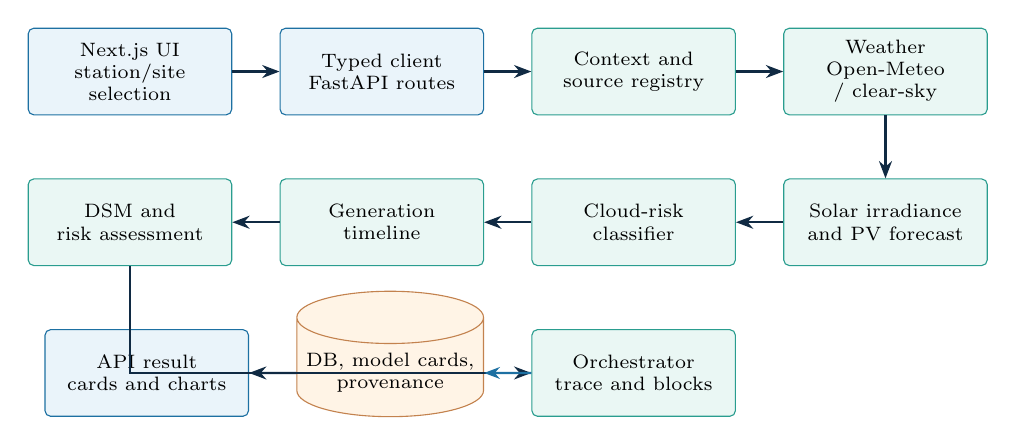
\begin{tikzpicture}[node distance=6mm]
\node[component] (ui) {Next.js UI\\station/site selection};
\node[component, right=of ui] (api) {Typed client\\FastAPI routes};
\node[agent, right=of api] (context) {Context and\\source registry};
\node[agent, right=of context] (weather) {Weather\\Open-Meteo / clear-sky};
\node[agent, below=8mm of weather] (solar) {Solar irradiance\\and PV forecast};
\node[agent, left=of solar] (cloud) {Cloud-risk\\classifier};
\node[agent, left=of cloud] (timeline) {Generation\\timeline};
\node[agent, left=of timeline] (dsm) {DSM and\\risk assessment};
\node[agent, below=8mm of cloud] (trace) {Orchestrator\\trace and blocks};
\node[store, left=of trace] (persist) {DB, model cards,\\provenance};
\node[component, left=of persist] (result) {API result\\cards and charts};

\draw[flow] (ui) -- (api);
\draw[flow] (api) -- (context);
\draw[flow] (context) -- (weather);
\draw[flow] (weather) -- (solar);
\draw[flow] (solar) -- (cloud);
\draw[flow] (cloud) -- (timeline);
\draw[flow] (timeline) -- (dsm);
\draw[flow] (dsm) |- (trace);
\draw[dataflow] (trace) -- (persist);
\draw[flow] (persist) -- (result);
\end{tikzpicture}}
\caption{Current implemented substation/site decision-support loop.}
\end{figure}

Current honest limits:

\begin{itemize}
  \item substation capacity is unavailable for all 344 OSM records;
  \item local measured PV and feeder/substation load are not connected;
  \item PV output is estimated from irradiance and configuration;
  \item official monetary DSM activation is pending source/version review;
  \item the production RL card remains blocked;
  \item authentication, tenant enforcement, alert delivery, read-only plant integration,
        HTTPS/operations evidence, and managed AWS deployment remain incomplete or unverified.
\end{itemize}

\section{Pull-Request and Branch Record}

\begin{longtable}{@{}C{1.2cm}L{5.2cm}L{5.0cm}L{3.5cm}@{}}
\caption{GitHub pull-request record relevant to main.}\label{tab:prs}\\
\toprule
\textbf{PR} & \textbf{Title / scope} & \textbf{Result} & \textbf{Main merge}\\
\midrule
\endfirsthead
\toprule
\textbf{PR} & \textbf{Title / scope} & \textbf{Result} & \textbf{Main merge}\\
\midrule
\endhead
\bottomrule
\endfoot
2 & Redis health and root path & merged & \code{016b41c}\\
3 & CI backend tests and frontend build & merged & \code{bb62673}\\
4 & Real Open-Meteo + pvlib nowcasting and DSM & merged & \code{f13bc3d}\\
5 & Harden CI/CD and Pages & merged & \code{8bb5e0a}\\
6 & Erbs fallback for GHI-only data & merged & \code{3950741}\\
7 & Settlement, energy balance, API agent, RL & merged & \code{70c75cd}\\
8 & Persistent DB, historical RL, new UI & merged & \code{56beb46}\\
9 & Karnataka/BESCOM, multi-year and current ingestion & merged & \code{6bb54f8}\\
10 & CodeRabbit-generated unit-test branch & open; not in main & side commit \code{32eec8a}\\
\end{longtable}

\section{Complete Main-Branch Commit Ledger}

\begin{footnotesize}
\begin{longtable}{@{}C{1.9cm}C{2.1cm}L{6.0cm}L{5.1cm}@{}}
\caption{All 37 commits on main, in chronological order.}\label{tab:commits}\\
\toprule
\textbf{Commit} & \textbf{Date} & \textbf{Repository summary} & \textbf{Implementation meaning}\\
\midrule
\endfirsthead
\toprule
\textbf{Commit} & \textbf{Date} & \textbf{Repository summary} & \textbf{Implementation meaning}\\
\midrule
\endhead
\bottomrule
\endfoot
\code{6d08097} & 20 Jun & Phase 1 complete MVP & Initial backend, frontend, agents, DSM/fuzzy risk, tests, docs\\
\code{957f146} & 20 Jun & Frontend UI overhaul & Dashboard, cards, deviation and timeline visuals\\
\code{d4b484f} & 20 Jun & Temporary-file cleanup & Repository hygiene\\
\code{7e46fd8} & 20 Jun & 3D SVG/glass UI & Solar, risk, energy visuals and theme\\
\code{6e85caf} & 20 Jun & GitHub Pages and mock engine & Static demonstration/deployment path\\
\code{e092af5} & 24 Jun & Cohesive dark glass UI & Design-system and page unification\\
\code{3627938} & 26 Jun & Redis health/root fix & Correct live health and root serving\\
\code{016b41c} & 26 Jun & Merge PR 2 & Integrated runtime fix\\
\code{b872d09} & 26 Jun & CI workflow & Backend tests and frontend build\\
\code{bb62673} & 26 Jun & Merge PR 3 & Integrated CI\\
\code{5054782} & 26 Jun & Real nowcasting + DSM & Open-Meteo, pvlib, real timeline, deterministic risk\\
\code{f13bc3d} & 26 Jun & Merge PR 4 & Integrated real nowcasting\\
\code{6d7cf77} & 26 Jun & Harden CI/CD and Pages & Ruff, artifact/live checks, deployment docs\\
\code{b283903} & 26 Jun & OpenAPI route test fix & FastAPI-version-stable route verification\\
\code{8bb5e0a} & 26 Jun & Merge PR 5 & Integrated hardened pipeline\\
\code{a107eea} & 26 Jun & Erbs GHI fallback & Physically valid DNI/DHI derivation\\
\code{3950741} & 26 Jun & Merge PR 6 & Integrated Erbs fallback\\
\code{02ed09a} & 26 Jun & Full platform foundation & Settlement, reward, energy, RL, API agent\\
\code{70c75cd} & 26 Jun & Merge PR 7 & Integrated full-platform modules\\
\code{5ce7bfe} & 27 Jun & Persistence, historical RL, new UI & DB, archive training, energy/settlement/RL pages\\
\code{56beb46} & 27 Jun & Merge PR 8 & Integrated persistent data/UI\\
\code{f30e504} & 27 Jun & Karnataka/BESCOM and current data & Multi-year/current ingestion and state workflow\\
\code{6bb54f8} & 27 Jun & Merge PR 9 & Integrated Karnataka expansion\\
\code{95fb856} & 6 Jul & Phase 1.7 real-data ML & Provenance-first datasets, agents, cards, honest gates\\
\code{507c6be} & 7 Jul & AWS IaC and documentation & ECS/RDS/Redis/S3/CloudFront intended stack\\
\code{1070a11} & 7 Jul & 2 GB host optimization & Small-instance Compose tuning\\
\code{d4c7e62} & 7 Jul & Ubuntu deploy script & One-command server deployment workflow\\
\code{5c158c1} & 7 Jul & Backend port 8080 & Host/proxy port alignment\\
\code{7c0f22e} & 7 Jul & Nginx proxy & Subdomain reverse-proxy attempt\\
\code{a17e3ef} & 7 Jul & Direct frontend fallback & Resolved port-80 conflict path\\
\code{04f61d5} & 7 Jul & Subdomain setup & Nginx site automation\\
\code{9b1c7eb} & 7 Jul & ML formatting & Ruff code-format cleanup\\
\code{9efbe28} & 7 Jul & Kaggle download helper & Dataset acquisition support\\
\code{16e6a4e} & 7 Jul & Kaggle pipeline/models/report & Four datasets/models, APIs, cards, evidence\\
\code{df372d2} & 7 Jul & History merge & Combined infrastructure and Kaggle lines\\
\code{360615f} & 7 Jul & Evidence-based final report & Hosted/repository verification and formula sources\\
\code{5bed3cd} & 7 Jul & Substation-driven workflow & Context, orchestration, endpoints, UI panel, 118-test baseline\\
\end{longtable}
\end{footnotesize}

\subsection{Fetched commits not in main}

\begin{itemize}
  \item \code{85c7753}: side-branch CI commit associated with the Redis/root-path branch history.
  \item \code{32eec8a}: CodeRabbit-generated tests on open PR 10; not merged into main.
\end{itemize}

\section{Current Verification Result}

On 9 July 2026, the current checkout was revalidated:

\begin{itemize}
  \item \code{python -m pytest tests -q}: \textbf{118 passed}.
  \item \code{python -m ruff check app tests}: \textbf{all checks passed}.
  \item \code{npm run build}: \textbf{compiled, linted, type-checked, and generated 16 pages}.
\end{itemize}

This verifies the current repository baseline. It does not automatically verify production
uptime, official regulatory interpretation, external datasets not committed to the repository,
managed AWS deployment, or real plant telemetry.

\clearpage
\part{Complete Execution and Agentic Architecture}

\section{Outcome and Scope}

The target is a production-capable solar decision-support platform that connects weather and
station data to forecast models, deterministic energy and DSM calculations, safe agentic
reasoning, operator workflows, and eventually validated plant telemetry. The system must answer:

\begin{enumerate}
  \item How much power can each DG or solar station generate over the selected horizon?
  \item How does the forecast compare with schedule, request, demand, and measured actuals?
  \item What energy gap, risk band, or regulatory DSM result follows?
  \item What should an operator review or do next, with complete provenance and calculation trace?
  \item Can a constrained RL policy improve advisory recommendations after real local outcomes exist?
\end{enumerate}

\begin{callout}{Dual truth model}
Every response has a deterministic truth plane and an optional reasoning plane. The truth plane
owns all source data, units, forecasts, formulas, model outputs, and money calculations. The
reasoning plane may route tools, summarize, detect inconsistencies, and recommend review actions.
It may never overwrite numeric results or invent missing values.
\end{callout}

\subsection{Four-level product model}

\begin{figure}[H]
\centering
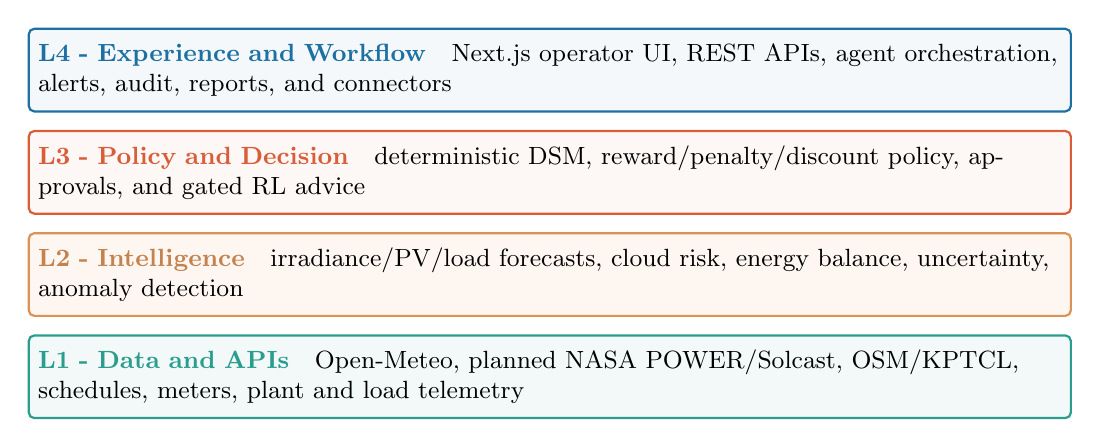
\begin{tikzpicture}[node distance=2.2mm]
\node[layer, draw=blue, fill=blue!5] (l4)
  {\textbf{\textcolor{blue}{L4 - Experience and Workflow}}\quad
  Next.js operator UI, REST APIs, agent orchestration, alerts, audit, reports, and connectors};
\node[layer, below=of l4, draw=red, fill=red!5] (l3)
  {\textbf{\textcolor{red}{L3 - Policy and Decision}}\quad
  deterministic DSM, reward/penalty/discount policy, approvals, and gated RL advice};
\node[layer, below=of l3, draw=amber!90!black, fill=amber!9] (l2)
  {\textbf{\textcolor{amber!80!black}{L2 - Intelligence}}\quad
  irradiance/PV/load forecasts, cloud risk, energy balance, uncertainty, anomaly detection};
\node[layer, below=of l2, draw=green, fill=green!6] (l1)
  {\textbf{\textcolor{green}{L1 - Data and APIs}}\quad
  Open-Meteo, planned NASA POWER/Solcast, OSM/KPTCL, schedules, meters, plant and load telemetry};
\end{tikzpicture}
\caption{The complete four-level SuryaGrid product model.}
\end{figure}

\section{Full Frontend-Backend-Agent Architecture}

\begin{figure}[H]
\centering
\resizebox{0.96\linewidth}{!}{
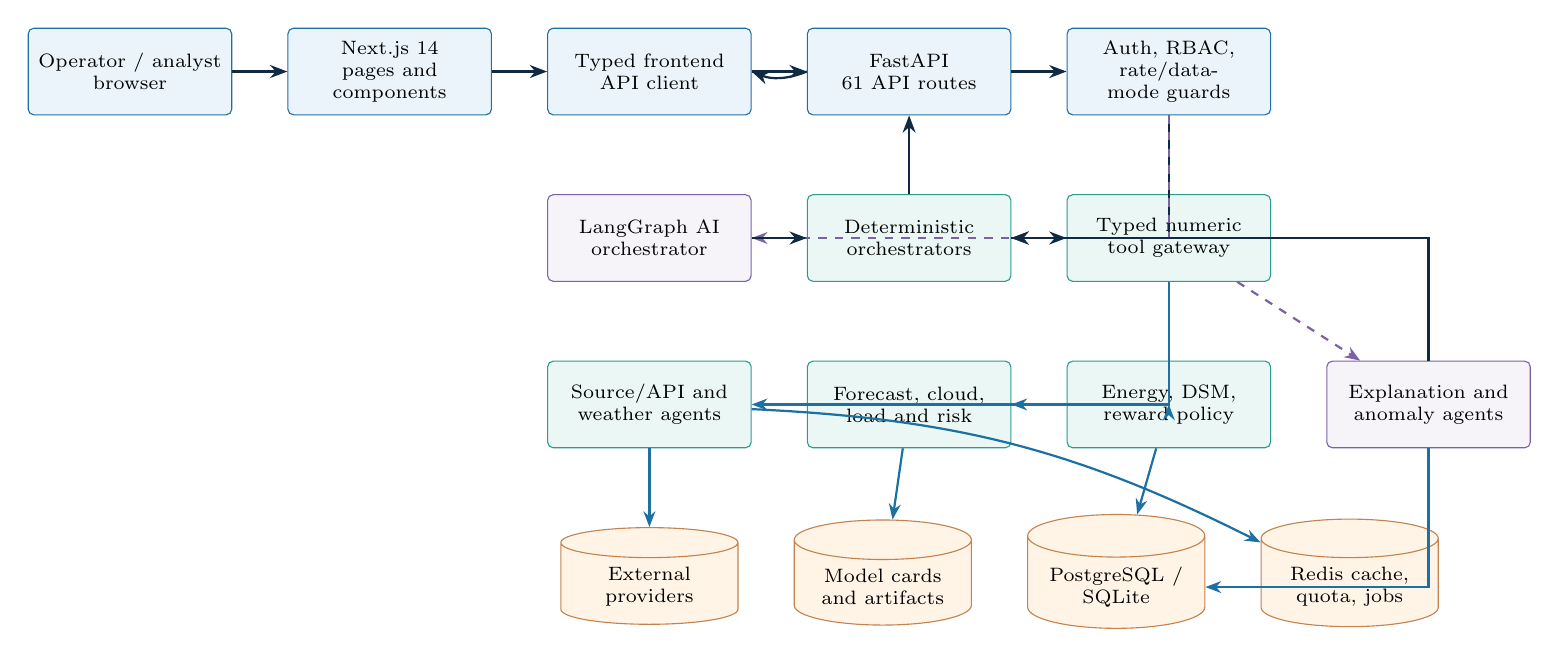
\begin{tikzpicture}[node distance=5mm and 7mm]
\node[component] (user) {Operator / analyst\\browser};
\node[component, right=of user] (next) {Next.js 14\\pages and components};
\node[component, right=of next] (client) {Typed frontend\\API client};
\node[component, right=of client] (fastapi) {FastAPI\\61 API routes};
\node[component, right=of fastapi] (guard) {Auth, RBAC,\\rate/data-mode guards};

\node[agent, below=10mm of fastapi] (orch) {Deterministic\\orchestrators};
\node[aiagent, left=of orch] (aiorch) {LangGraph AI\\orchestrator};
\node[agent, right=of orch] (tools) {Typed numeric\\tool gateway};

\node[agent, below=10mm of aiorch] (source) {Source/API and\\weather agents};
\node[agent, right=of source] (forecast) {Forecast, cloud,\\load and risk};
\node[agent, right=of forecast] (logic) {Energy, DSM,\\reward policy};
\node[aiagent, right=of logic] (explain) {Explanation and\\anomaly agents};

\node[store, below=10mm of source] (providers) {External\\providers};
\node[store, right=of providers] (models) {Model cards\\and artifacts};
\node[store, right=of models] (db) {PostgreSQL /\\SQLite};
\node[store, right=of db] (redis) {Redis cache,\\quota, jobs};

\draw[flow] (user) -- (next);
\draw[flow] (next) -- (client);
\draw[flow] (client) -- (fastapi);
\draw[flow] (fastapi) -- (guard);
\draw[flow] (guard) |- (orch);
\draw[aiflow] (guard) |- (aiorch);
\draw[flow] (aiorch) -- (orch);
\draw[flow] (orch) -- (tools);
\draw[dataflow] (tools) |- (source);
\draw[dataflow] (tools) |- (forecast);
\draw[dataflow] (tools) |- (logic);
\draw[aiflow] (tools) -- (explain);
\draw[dataflow] (source) -- (providers);
\draw[dataflow] (forecast) -- (models);
\draw[dataflow] (logic) -- (db);
\draw[dataflow] (source) to[bend left=12] (redis);
\draw[dataflow] (explain) |- (db);
\draw[flow] (explain.north) |- (orch.east);
\draw[flow] (orch.north) -- (fastapi.south);
\draw[flow] (fastapi.west) to[bend left=22] (client.east);
\end{tikzpicture}}
\caption{Target connection architecture. Solid navy paths are request/control; blue paths carry
typed data; dashed violet paths are optional LLM reasoning.}
\end{figure}

\subsection{Connection contract}

\begin{enumerate}
  \item The UI calls only the typed client in \code{frontend/lib/api.ts}; pages do not call
        providers or model files directly.
  \item FastAPI validates request identity, role, site scope, data mode, units, and schema.
  \item The deterministic orchestrator remains the production fallback and numerical authority.
  \item The optional LangGraph route chooses from an allowlist of typed tools; tools call existing
        providers, models, energy services, and DSM engines.
  \item Tool output is immutable and hashed into the trace before an LLM sees it.
  \item The LLM returns schema-validated routing, explanation, anomaly, or escalation fields.
  \item Persistence stores inputs, source IDs, model/formula/policy versions, outputs, agent trace,
        calculation trace, latency, cost, and approval status.
  \item The API returns one stable response envelope to the UI. If LLM service is unavailable,
        numeric output still completes and the explanation is marked unavailable or deterministic.
\end{enumerate}

\section{Frontend to Backend Connection Matrix}

\begin{footnotesize}
\begin{longtable}{@{}L{2.3cm}L{3.3cm}L{4.4cm}L{4.4cm}@{}}
\caption{Frontend pages, backend contracts, and agent ownership.}\label{tab:frontback}\\
\toprule
\textbf{Frontend surface} & \textbf{Primary client calls} & \textbf{Backend route groups} &
\textbf{Agents/services}\\
\midrule
\endfirsthead
\toprule
\textbf{Frontend surface} & \textbf{Primary client calls} & \textbf{Backend route groups} &
\textbf{Agents/services}\\
\midrule
\endhead
\bottomrule
\endfoot
Dashboard & health, predict, orchestrate substation, generation timeline &
\code{/health}, \code{/predict}, \code{/orchestrate/substation}, \code{/generation/timeline} &
orchestrator, substation orchestrator, forecast, risk, explanation\\
Locations & catalog, context, nearest, coverage &
\code{/substations/*}, \code{/locations/*}, \code{/sites/*/data-coverage} &
location data, source registry, substation context\\
Predictions & predict site, forecast, model status &
\code{/predict/*}, \code{/forecast/*}, \code{/ml/model/status} &
forecast, feature engineering, model registry\\
Timeline & timeline, summary, generation timeline &
\code{/timeline/*}, \code{/summary/*}, \code{/generation/timeline} &
forecast, energy, DSM classifier\\
Energy & energy and consumption profiles &
\code{/energy/*}, \code{/consumption/profiles} &
energy service, forecast, consumption service\\
DSM & profiles, advanced check, substation DSM, Karnataka DSM &
\code{/dsm/*}, \code{/dsm/forecast}, \code{/dsm/karnataka/*} &
DSM classifier, DSM engine, reward/policy\\
Settlement & settle day, settlement history, RL rates &
\code{/settle*}, \code{/settlements/*}, \code{/rl/rates} &
reward, persistence, energy/DSM services\\
RL Lab & train, rates, run history &
\code{/rl/train}, \code{/rl/rates}, \code{/rl/runs} &
RL environment/trainer, persistence; production use gated\\
ML & ingest, build, train, predict, status &
\code{/ml/*}, \code{/kaggle/*} &
Kaggle data, feature engineering, model registry\\
Data Sources & source catalog, provider status &
\code{/sources/*}, \code{/data-sources/status}, \code{/providers/status} &
source registry, API management, live weather\\
Karnataka & regions, seed, BESCOM status, Karnataka DSM &
\code{/karnataka/*}, \code{/bescom/status}, \code{/dsm/karnataka/*} &
location, BESCOM connector framework, DSM engine\\
System & health, system status, agent/data status &
\code{/health}, \code{/system/status}, \code{/agents/*} &
API management, source registry, all status providers\\
\end{longtable}
\end{footnotesize}

\section{Agentic Architecture and Agent Inventory}

\subsection{Current deterministic and ML agents}

\begin{footnotesize}
\begin{longtable}{@{}L{3.1cm}L{4.5cm}L{4.1cm}L{3.0cm}@{}}
\caption{Existing agent modules and target role.}\label{tab:currentagents}\\
\toprule
\textbf{Module} & \textbf{Responsibility} & \textbf{Connects to} & \textbf{Status}\\
\midrule
\endfirsthead
\toprule
\textbf{Module} & \textbf{Responsibility} & \textbf{Connects to} & \textbf{Status}\\
\midrule
\endhead
\bottomrule
\endfoot
\code{api_agent.py} & provider choice, failover, quota state & providers, Redis, orchestrator & \stPartial\\
\code{api_management_agent.py} & provider health, retry, rate visibility & system/status routes & \stPartial\\
\code{source_registry_agent.py} & source records and formula references & registry, provenance, UI & \stImpl\\
\code{live_weather_agent.py} & live weather and labelled fallback & Open-Meteo, Redis, DB & \stImpl\\
\code{kaggle_data_agent.py} & Kaggle ingestion and normalization & data pipeline and model builds & \stImpl\\
\code{location_data_agent.py} & locations, substations, coverage & OSM parquet, site services & \stImpl\\
\code{feature_engineering_agent.py} & quality checks and model features & dataset builder, ML models & \stImpl\\
\code{forecast_agent.py} & formula/ML/hybrid solar nowcast & weather, pvlib, model registry & \stImpl\\
\code{dsm_classifier_agent.py} & interval deviation classification & schedule, forecast/actual & \stImpl\\
\code{dsm_engine_agent.py} & rule-profile resolution and persistence & DSM repository and policy & \stPartial\\
\code{risk_agent.py} & deterministic operational risk & forecast and DSM output & \stImpl\\
\code{fuzzy_risk_agent.py} & fuzzy risk inference & forecast/DSM features & \stImpl\\
\code{reward_agent.py} & reward/penalty/discount research engine & settlement and RL & \stGate\\
\code{explanation_agent.py} & deterministic explanation text & final result envelope & \stImpl\\
\code{persistence_agent.py} & saves important records & DB repository and audit & \stImpl\\
\code{orchestrator_agent.py} & standard interval sequence & all numeric agents & \stImpl\\
\code{substation_orchestrator.py} & substation-driven seven-step flow & context, weather, ML, DSM & \stImpl\\
\end{longtable}
\end{footnotesize}

\subsection{Planned LLM reasoning agents}

\begin{longtable}{@{}L{3.1cm}L{4.8cm}L{4.1cm}L{2.4cm}@{}}
\caption{New agentic reasoning layer.}\label{tab:aiagents}\\
\toprule
\textbf{Agent} & \textbf{Allowed responsibility} & \textbf{Forbidden responsibility} &
\textbf{Fallback}\\
\midrule
\endfirsthead
\toprule
\textbf{Agent} & \textbf{Allowed responsibility} & \textbf{Forbidden responsibility} &
\textbf{Fallback}\\
\midrule
\endhead
\bottomrule
\endfoot
AI Orchestrator & select approved tools, route around missing inputs, request review,
explain routing & changing numeric outputs, tariffs, schedules, or control set-points &
deterministic orchestrator\\
AI Explanation & structured summary, evidence-linked narrative, operator recommendations &
inventing causes, values, regulations, or confidence & deterministic explanation\\
Anomaly Detective & interpret deterministic anomaly flags, group incidents, suggest investigation &
being the only detector or suppressing hard-rule alerts & rule-based detector\\
\end{longtable}

\subsection{LangGraph execution design}

Use a typed \code{StateGraph} with explicit START/END, conditional edges, durable checkpoints,
bounded retries, and interrupt points for human approval. The design is:

\begin{enumerate}
  \item \textbf{Analyze context:} deterministic validation creates allowed/missing/blocked fields.
  \item \textbf{Choose tools:} AI orchestrator selects only tools whose prerequisites are present.
  \item \textbf{Execute tools:} numeric tools run outside the model and return typed results.
  \item \textbf{Validate:} schema, unit, bounds, provenance, and output hash checks run.
  \item \textbf{Assess anomaly:} hard rules/statistics flag anomalies; LLM adds explanation only.
  \item \textbf{Apply policy:} deterministic effective-dated DSM/reward profile runs.
  \item \textbf{Interrupt if required:} unsupported money, low confidence, policy change, or control
        recommendation requires a human decision.
  \item \textbf{Synthesize:} explanation agent returns strict JSON fields.
  \item \textbf{Persist and publish:} state/checkpoint, audit, costs, and final envelope are saved.
\end{enumerate}

\subsection{Shared state and communication protocol}

\begin{footnotesize}
\begin{longtable}{@{}L{3.1cm}L{7.0cm}L{4.4cm}@{}}
\caption{Minimum shared state contract.}\label{tab:state}\\
\toprule
\textbf{State group} & \textbf{Required fields} & \textbf{Writer}\\
\midrule
\endfirsthead
\toprule
\textbf{State group} & \textbf{Required fields} & \textbf{Writer}\\
\midrule
\endhead
\bottomrule
\endfoot
Identity & trace ID, user/role, tenant, station/site, request timestamp & API guard\\
Context & coordinates, timezone, units, capacity, schedule, policy ID, missing fields &
context service\\
Sources & source IDs, retrieval time, license, raw hash, fallback and quality status &
source/API agents\\
Forecast & GHI/PV/load intervals, confidence, model/formula versions & forecast tools\\
Decision & measured actual, schedule deviation, energy gap, DSM band/amount, blocked fields &
logic and policy tools\\
Reasoning & route decision, explanation JSON, anomalies, recommended review & LLM agents\\
Governance & approval, interrupt reason, retry count, token/cost, latency, final status &
orchestrator and persistence\\
\end{longtable}
\end{footnotesize}

Agent-to-agent communication uses state, not free-form hidden conversation. Every node appends an
event to \code{agent_trace}; every numeric result appends source/formula/model details to
\code{calculation_trace}. Errors are typed as retryable, fallback-eligible, review-required, or
blocked. No agent may silently convert a blocked result into a value.

\section{Data, Models, Policy, and Source Plan}

\subsection{Provider and data priorities}

\begin{longtable}{@{}L{3.0cm}L{3.0cm}L{5.0cm}L{3.5cm}@{}}
\caption{Data and policy integration priority.}\label{tab:sourcesplan}\\
\toprule
\textbf{Source/work} & \textbf{Current state} & \textbf{Planned implementation} &
\textbf{Required gate}\\
\midrule
\endfirsthead
\toprule
\textbf{Source/work} & \textbf{Current state} & \textbf{Planned implementation} &
\textbf{Required gate}\\
\midrule
\endhead
\bottomrule
\endfoot
Open-Meteo & live weather and archive & retain as primary weather provider &
provider SLO and cache\\
NASA POWER & historical cross-check only & runtime historical/NRT fallback provider,
not a day-ahead forecast substitute & latency/freshness test\\
Solcast & not integrated & optional contracted forecast provider & contract, quota, cost\\
NPP/Grid India reports & public reports confirmed & feasibility parser for region/state
generation and capacity; do not assume hourly Karnataka load until inspected & schema proof\\
KPTCL/Aikosh candidate & not verified in repo & inspect access, fields, licensing, current vs
planned capacity, then match conservatively & source and match review\\
Local PV actuals & absent & KPCL/BESCOM/operator data agreement and ingestion contract &
meter semantics and consent\\
KERC 2026 DSM & externally reported; not encoded from archived official source &
effective-dated cumulative slab engine with source snapshot & official gazette + legal review\\
Load model & India-wide, non-production locally & train regional then Karnataka/site model &
chronological holdout and domain review\\
RL policy & production blocked & offline constrained research then advisory shadow mode &
real outcomes + approved economics\\
\end{longtable}

\subsection{KERC 2026 handling}

Published reports describe a solar tolerance band of 5\%, cumulative charges of Rs.~0.25,
Rs.~0.50, and Rs.~0.75 per unit across increasing deviation slabs, a scheduled-generation
denominator, a deemed 1 MW schedule for zero-schedule injection, and an annual cap of 3 paise
per unit times annual generation. These values are \textbf{requirements candidates}, not yet
permission to emit settlement money.

Before \code{emits_rupee_values=true}:

\begin{enumerate}
  \item archive the official Gazette/KERC document and checksum it;
  \item record notification date, effective date, applicability, section/table references,
        amendment status, and legal reviewer;
  \item implement cumulative slab arithmetic, annual cap, interval aggregation, zero-schedule
        handling, over/under-generation treatment, and version selection;
  \item independently reproduce golden cases and compare against a manual worksheet;
  \item add dual approval, rollback, and audit for rule activation.
\end{enumerate}

\section{Security, Reliability, and AI Guardrails}

\begin{itemize}
  \item OIDC/JWT authentication, RBAC, tenant and site isolation on every protected route.
  \item Secret manager for provider and OpenRouter keys; never expose keys to browser or logs.
  \item Request rate limits plus separate LLM token, spend, and concurrency budgets.
  \item Tool allowlists, JSON Schema output, prompt-injection filtering, and no arbitrary code tools.
  \item Deterministic numeric equivalence test: AI and non-AI routes return identical numeric fields.
  \item Model/provider pinning with explicit fallback list and recorded final model ID.
  \item LLM outage, timeout, malformed output, and budget exhaustion fall back deterministically.
  \item Human interrupts for money activation, rule changes, low-confidence recommendations,
        external messages, or any future control action.
  \item Immutable audit: prompt template version, tool inputs/outputs, response schema, token usage,
        latency, reviewer, and release version.
  \item HTTPS, backups, restore drills, provider outage tests, SLOs, data drift, model drift,
        and incident runbooks before pilot.
\end{itemize}

\section{Detailed Execution Roadmap}

\textbf{Implementation status (this iteration).} Phases 0--4 have been implemented in
code behind honest gates; every external-data dependency (official KERC tariff,
KPTCL/CEA capacity, SLDC load, measured local PV) remains blocked and is represented
by validated-but-empty machinery rather than fabricated values. Test coverage added:
\code{test\_phase0\_foundation.py} (6), \code{test\_phase1\_providers\_kerc.py} (11),
\code{test\_ai\_reasoning\_layer.py} (7), \code{test\_phase2\_data\_pipeline.py} (9),
\code{test\_phase3\_model\_rl\_gates.py} (4), \code{test\_phase4\_auth\_alerts\_connector.py}
(10). Phase 5 (controlled pilot) remains future work pending pilot-site data access.

\subsection{Phase 0 - Foundation hardening (Week 1)} \textbf{[DONE]}

\textbf{Work items}
\begin{enumerate}
  \item Enforce \code{APP_DATA_MODE} on every API and background job. Real mode forbids silent
        synthetic fallback; clear-sky physics is labelled separately.
  \item Unify the source registry and model-card provenance into one \code{SourceRecord} contract.
  \item Verify Docker Compose end-to-end, health checks, migrations, backend tests, frontend build,
        and evidence log.
  \item Quarantine unsupported monetary defaults and add a test that forbids unapproved currency.
\end{enumerate}

\textbf{Deliverables:} data-mode behavior matrix, unified registry, no-orphan-source tests,
Docker verification log, and unchanged 118-test baseline or better.

\subsection{Phase 1 - Provider and regulation integration (Weeks 2--3)} \textbf{[DONE, gated]}

\textbf{NASA POWER}
\begin{itemize}
  \item Add \code{app/providers/nasa_power.py} behind \code{WeatherProvider}.
  \item Map GHI, temperature, humidity, wind, and pressure; use explicit UTC/LST conversion.
  \item Cache responses, record freshness, and use it for historical fill/NRT fallback.
  \item Cross-validate against Open-Meteo; never call reanalysis a live forecast.
\end{itemize}

\textbf{KERC rule parser}
\begin{itemize}
  \item Add effective-dated \code{kerc_dsm_2026.py} only after the official-source gate.
  \item Support cumulative slabs, annual cap, deemed schedule, applicability, and source citations.
  \item Add scenario tests, manual reproduction, frontend attribution, and rollback.
\end{itemize}

\subsection{Phase 1.5 - Real agentic reasoning layer (Weeks 3--4)} \textbf{[DONE]}

\begin{itemize}
  \item Add \code{langgraph}, \code{langchain-core}, and the selected OpenAI-compatible client.
  \item Create \code{app/agents/ai/state.py}, \code{tools.py}, \code{orchestrator.py},
        \code{explanation.py}, \code{anomaly_detective.py}, prompts, and policies.
  \item Add \code{/api/v1/orchestrate/substation/ai} beside the deterministic route.
  \item Add strict structured output, durable checkpointing, retry limits, and approval interrupts.
  \item Add \code{AIInsightsPanel}, anomaly/alert UI, and reasoning trace display.
  \item Prove numeric equivalence and deterministic fallback under LLM failure.
\end{itemize}

\subsection{Phase 2 - Data acquisition and enrichment (Weeks 5--6)} \textbf{[SCHEMA/PARSER DONE; external data blocked]}

\begin{itemize}
  \item Inspect NPP/Grid India report files before defining granularity; build fixture-driven parser.
  \item Obtain regional/Karnataka load from a source that actually exposes required intervals.
  \item Inspect KPTCL/Aikosh or official KPTCL/CEA capacity sources; distinguish planned augmentation
        from commissioned capacity.
  \item Match stations by normalized name, operator, voltage, and geography with manual review.
  \item Begin local PV data requests to KPCL, BESCOM, and willing plant operators.
  \item Prepare a local-PV ingestion schema for timestamp, AC/DC power, irradiance, inverter state,
        quality flag, and meter provenance.
\end{itemize}

\subsection{Phase 3 - Model rebuild and gated RL (Weeks 7--10)} \textbf{[GATES AUDITED; RL stays blocked]}

\begin{itemize}
  \item Train regional load with chronological splits and compare against the national baseline.
  \item Train site-level PV only when measured site truth and configuration are sufficient.
  \item Calibrate intervals, bias, drift, and seasonal/site performance; produce model cards.
  \item Build an RL environment from approved data. Estimated PV may support research but can never
        make the policy production-ready.
  \item Compare RL with no-action and deterministic baselines; require zero safety violations.
  \item Promote agent status only when its own evidence and acceptance gate passes.
\end{itemize}

\subsection{Phase 4 - Product integration and hardening (Weeks 10--14)} \textbf{[DONE, flag-gated; deploy verify host-blocked]}

\begin{itemize}
  \item Complete OIDC/JWT, RBAC, tenant isolation, rate limits, audit, and spend controls.
  \item Make station selection a shared frontend context that drives every relevant page/card.
  \item Add alerts, acknowledgment, explanation provenance, and blocked-reason UX.
  \item Implement one read-only plant connector and a replay environment; no control commands.
  \item Verify HTTPS, actual deployment topology, backups, restore, CI/CD, metrics, traces, and SLOs.
\end{itemize}

\subsection{Phase 5 - Controlled pilot (Weeks 15--22)} \textbf{[FUTURE - needs pilot-site data access]}

\begin{itemize}
  \item Run a 1--3-site shadow pilot for at least 2--4 weeks.
  \item Compare forecast, schedule, measured actual, policy result, and operator decision.
  \item Review every alert, blocked result, model drift event, and LLM fallback.
  \item If RL passed its gate, show advice only; record human acceptance/rejection and outcome.
  \item Conduct incident, provider outage, backup/restore, policy rollback, and security drills.
  \item Hold a go/extend/stop production-readiness review with accepted residual risks.
\end{itemize}

\section{Timeline and Milestones}

\begin{figure}[H]
\centering
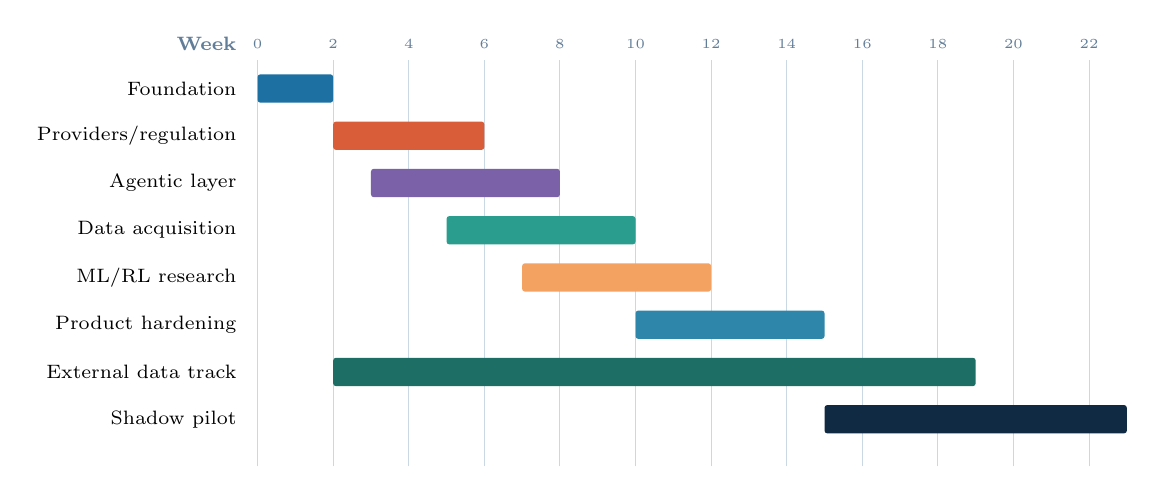
\begin{tikzpicture}[x=0.48cm,y=0.60cm]
\def\xoff{5.6}
\foreach \w in {0,2,...,22} {
  \draw[grid,thin] (\xoff+\w,0.2) -- (\xoff+\w,8.8);
  \node[font=\tiny,text=muted] at (\xoff+\w,9.15) {\w};
}
\node[font=\scriptsize\bfseries,text=muted,anchor=east] at (\xoff-0.3,9.15) {Week};
\node[font=\scriptsize,anchor=east] at (\xoff-0.3,8.2) {Foundation};
\fill[blue,rounded corners=1pt] (\xoff,7.9) rectangle (\xoff+2,8.5);
\node[font=\scriptsize,anchor=east] at (\xoff-0.3,7.2) {Providers/regulation};
\fill[red,rounded corners=1pt] (\xoff+2,6.9) rectangle (\xoff+6,7.5);
\node[font=\scriptsize,anchor=east] at (\xoff-0.3,6.2) {Agentic layer};
\fill[violet,rounded corners=1pt] (\xoff+3,5.9) rectangle (\xoff+8,6.5);
\node[font=\scriptsize,anchor=east] at (\xoff-0.3,5.2) {Data acquisition};
\fill[green,rounded corners=1pt] (\xoff+5,4.9) rectangle (\xoff+10,5.5);
\node[font=\scriptsize,anchor=east] at (\xoff-0.3,4.2) {ML/RL research};
\fill[amber,rounded corners=1pt] (\xoff+7,3.9) rectangle (\xoff+12,4.5);
\node[font=\scriptsize,anchor=east] at (\xoff-0.3,3.2) {Product hardening};
\fill[cyan,rounded corners=1pt] (\xoff+10,2.9) rectangle (\xoff+15,3.5);
\node[font=\scriptsize,anchor=east] at (\xoff-0.3,2.2) {External data track};
\fill[green!70!black,rounded corners=1pt] (\xoff+2,1.9) rectangle (\xoff+19,2.5);
\node[font=\scriptsize,anchor=east] at (\xoff-0.3,1.2) {Shadow pilot};
\fill[navy,rounded corners=1pt] (\xoff+15,0.9) rectangle (\xoff+23,1.5);
\end{tikzpicture}
\caption{Integrated engineering and controlled-pilot schedule. The 10-week build track is inside
the 22-week evidence and pilot track.}
\end{figure}

\begin{footnotesize}
\begin{longtable}{@{}L{1.5cm}L{4.2cm}L{6.4cm}L{2.5cm}@{}}
\caption{Milestones and decision gates.}\label{tab:milestones}\\
\toprule
\textbf{Week} & \textbf{Milestone} & \textbf{Success criterion} & \textbf{Decision}\\
\midrule
\endfirsthead
\toprule
\textbf{Week} & \textbf{Milestone} & \textbf{Success criterion} & \textbf{Decision}\\
\midrule
\endhead
\bottomrule
\endfoot
1 & M0 Foundation & real-mode audit, registry design, Docker evidence, all tests/build pass &
engineering gate\\
3 & M1 Providers/rules & NASA provider validated; KERC source archived and golden cases reviewed &
source/legal gate\\
4 & M2 Agentic route & AI route returns schema-valid reasoning and identical numeric output;
fallback proven & safety gate\\
6 & M3 Data feasibility & inspected source files; coverage, interval, license, and quality report &
data gate\\
10 & M4 Model/RL research & signed model cards; RL beats baseline offline with zero safety breach &
research gate\\
14 & M5 Pilot-ready & auth/isolation, UI connection, read-only connector, SLO/restore drills &
operational gate\\
22 & M6 Pilot decision & shadow metrics, operator sign-off, incidents and residual risks reviewed &
go/extend/stop\\
\end{longtable}
\end{footnotesize}

\section{Standard Implementation Workflow}

Every roadmap item follows the same evidence chain:

\begin{figure}[H]
\centering
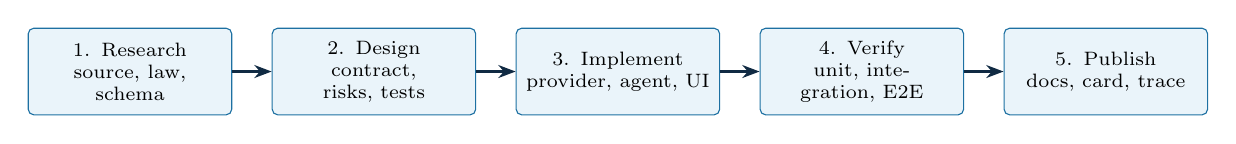
\begin{tikzpicture}[node distance=5mm]
\node[component] (research) {1. Research\\source, law, schema};
\node[component, right=of research] (design) {2. Design\\contract, risks, tests};
\node[component, right=of design] (implement) {3. Implement\\provider, agent, UI};
\node[component, right=of implement] (verify) {4. Verify\\unit, integration, E2E};
\node[component, right=of verify] (publish) {5. Publish\\docs, card, trace};
\draw[flow] (research) -- (design);
\draw[flow] (design) -- (implement);
\draw[flow] (implement) -- (verify);
\draw[flow] (verify) -- (publish);
\end{tikzpicture}
\caption{Required implementation workflow for every change.}
\end{figure}

\section{Testing and Acceptance}

\begin{itemize}
  \item \textbf{Regression:} current 118 tests, Ruff, and frontend build remain green.
  \item \textbf{Provider contract:} fixtures, timezones, units, missing data, retries, cache, drift.
  \item \textbf{Policy:} official-source golden cases, boundaries, cumulative slabs, cap, rollback.
  \item \textbf{Agentic:} tool allowlist, prompt injection, structured output, numeric equivalence,
        deterministic fallback, checkpoint/resume, human interrupt, spend limit.
  \item \textbf{Data quality:} coverage, freshness, duplicates, gaps, license, geography, domain shift.
  \item \textbf{ML:} chronological holdout, baseline comparison, calibration, season/site slices, drift.
  \item \textbf{RL:} offline only, deterministic baseline, stress cases, constraints, no unsafe action.
  \item \textbf{Frontend/backend:} contract tests for all client functions and page workflows.
  \item \textbf{Security/operations:} auth, tenant isolation, secrets, rate limits, HTTPS, restore,
        provider outage, rollback, load, SLO and incident drills.
\end{itemize}

\section{Cost and Capacity Planning}

Do not hardcode current model prices or model IDs in application logic. Select models from a
capability policy that requires tool calling, structured output, latency, geography/privacy,
availability, and budget. Record the actual model returned by the provider.

For planning:

\[
\text{daily LLM cost} =
\sum_a \left(
  \text{calls}_a \times
  \frac{\text{input tokens}_a \times p_{in,a} +
        \text{output tokens}_a \times p_{out,a}}{10^6}
\right)
\]

The supplied usage assumption of roughly 50 orchestrations, 50 explanations, and 24 anomaly
reviews per day is a \textbf{pilot scenario}, not measured traffic. Add cache-hit rate, retries,
provider fallback, and a 30--50\% contingency. Set daily and monthly hard budgets; when exhausted,
fall back to deterministic output.

\section{Risks and Honest End State}

\begin{footnotesize}
\begin{longtable}{@{}L{3.6cm}L{4.1cm}L{6.9cm}@{}}
\caption{Principal execution risks.}\label{tab:risks}\\
\toprule
\textbf{Risk} & \textbf{Effect} & \textbf{Response}\\
\midrule
\endfirsthead
\toprule
\textbf{Risk} & \textbf{Effect} & \textbf{Response}\\
\midrule
\endhead
\bottomrule
\endfoot
Official KERC text or interpretation changes & wrong monetary output &
effective-dated rules, archived source, legal review, no-money default, rollback\\
NPP files lack required load granularity & load pipeline blocked &
inspect first; obtain SLDC/site agreement; do not interpolate false hourly truth\\
Capacity dataset is planned work, not commissioned state & wrong station loading &
source classification, commissioning evidence, confidence and manual review\\
Local PV partnership fails & no production PV/RL validation &
retain estimate label; continue decision-support pilot without production RL\\
LLM changes numbers or invents evidence & unsafe decisions &
typed tools, immutable outputs, strict JSON, equivalence tests, deterministic fallback\\
Prompt injection or secret leakage & data/security incident &
allowlists, input separation, no secret in prompts, output validation, audit\\
Provider/model price or availability changes & cost/outage &
model policy, pinned tested options, fallback list, budgets, cache\\
Frontend and backend contracts diverge & broken operator workflow &
generated schemas, contract tests, one shared station context, CI build gate\\
Managed AWS is assumed deployed from Terraform & false readiness claim &
verify actual topology; label code-only infrastructure until observed\\
\end{longtable}
\end{footnotesize}

After the plan, the system may still honestly report the following as pending: real-time
KPTCL/SLDC telemetry without an agreement, on-site pyranometer validation, full local PV and load
coverage, inter-state CERC settlement handling, autonomous control, and production RL. These are
not documentation failures; they are evidence gates.

\section{Immediate Team Actions}

\begin{enumerate}
  \item Approve this architecture and make it the source of truth for implementation.
  \item Run the route-by-route \code{APP_DATA_MODE} and unsupported-currency audits.
  \item Verify Docker Compose and record container evidence.
  \item Implement NASA POWER as a historical/NRT fallback with explicit freshness semantics.
  \item Archive and legally review the official KERC 2026 source before enabling any rupee output.
  \item Create the typed LangGraph state/tool contracts and a deterministic-equivalence test first.
  \item Inspect candidate NPP and KPTCL/Aikosh files before committing to schemas or schedules.
  \item Send local PV data requests immediately because this is the longest external dependency.
\end{enumerate}

\section{External Technical References}

\begin{itemize}
  \item GitHub repository: \url{https://github.com/DBIT-Banglore/SuryaGrid}
  \item LangGraph: \url{https://github.com/langchain-ai/langgraph}
  \item OpenRouter API: \url{https://openrouter.ai/docs/api/reference/overview}
  \item OpenRouter tool calling: \url{https://openrouter.ai/docs/guides/features/tool-calling}
  \item NASA POWER temporal API: \url{https://power.larc.nasa.gov/docs/services/api/temporal/}
  \item National Power Portal published reports: \url{https://www.npp.gov.in/publishedReports}
  \item Karnataka Electricity Regulatory Commission: \url{https://kerc.karnataka.gov.in/}
\end{itemize}


\end{document}
